\section{Algorithm Testing}
\label{sec:algorithm_testing}

We can now proceed to test the algorithms we have implemented in the previous section.
In the following, the maps scenarios adopted are presented first, and then the results of the tests are shown.

\subsection{Map scenarios}
\label{subsec:map_scenarios}

Figures \ref{fig:test_maps} show the four image maps used to test the algorithm.
Even if the images here below are of size $300\text{x}300$, we preferred to scale down to $30\text{x}30$ in order to have a direct comparison between the results obtained previously with the grid-based algorithms.
Notice also that while the white areas are free space, the one marked in black or gray are to be considered as obstacles.
Finally, the green dot is the starting point of the vehicle, while the red one is the goal.

\begin{figure}[H]
    \centering
    \frame{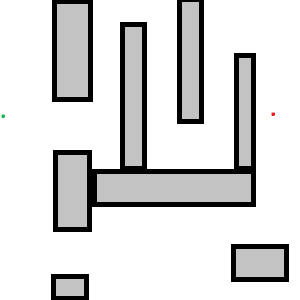
\includegraphics[width=0.48\textwidth]{./img/01.png}}
    \hspace{6pt}
    \frame{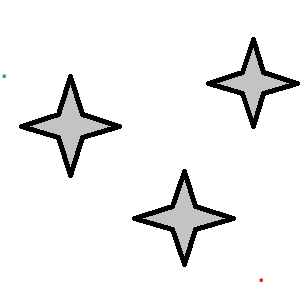
\includegraphics[width=0.48\textwidth]{./img/02.png}}

    \vspace{11pt}

    \frame{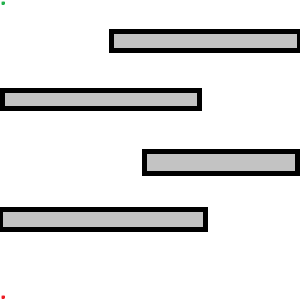
\includegraphics[width=0.48\textwidth]{./img/03.png}}
    \hspace{6pt}
    \frame{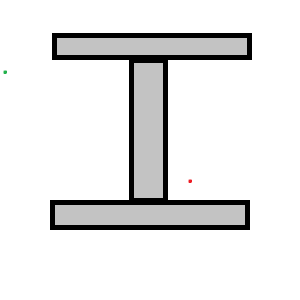
\includegraphics[width=0.48\textwidth]{./img/04.png}}
    \caption{Test maps used for the algorithm testing.}
    \label{fig:test_maps}
\end{figure}

\subsection{Results analysis}
\label{subsec:results_analysis}

In the following, results obtained running both RRT, RRT* and RRT kinematic algorithms on each of the scenario are presented.
For comparison purposes, the results obtained running the A* algorithm on the same maps are also reported, even if an in-depth analysis of the differences and performances of the two families of algorithms is left to the next section (Section \ref{sec:grid_vs_sample_based_planning}).

The plotting of both the (geometrical) connected graph and the best path found is also shown.
Tables presenting the main metrics of the tests are also shown.
The metrics are the following:

\begin{itemize}
    \item \textbf{Elapsed time}: here only the time needed to run the searching algorithm is considered (i.e. we are including the tree generation but excluding the plotting of the results);
    \item \textbf{Tree dimension}: number of nodes in the tree generated by the algorithm. In case of the A* algorithm, this is the number of nodes in the graph generated during the discretization/grid generation phase;
    \item \textbf{Path length}: length of the path found by the algorithm. This also correspond to the path cost, given that the cost of each edge is equal to its geometrical length.
\end{itemize}

Notice that the due to the randomness nature of sampling-based algorithms, the reported results must be interpreted as an average of 5 runs of each algorithm on each map.
Moreover, the tuning parameters of the algorithms such as step size and rewiring radius have been set on all the algorithms variants to be:

\begin{table}[H]
    \centering
    \begin{tabular}{|c|c|}
        \hline
        \textbf{Parameter} & \textbf{Value} \\
        \hline
        Step size          & 1.0            \\
        Rewiring radius*   & 1.5            \\
        \hline
    \end{tabular}
    \caption{Tuning parameters of the algorithms. The rewiring radius is only used in the RRT* algorithm.}
    \label{tab:algorithm_parameters}
\end{table}

Units are considered to be in pixels dimensions, where we recall the size of the map to be $30\text{x}30$.


\subsubsection{Map 1}
\label{subsec:map_1}

Results obtained running the three algorithms on the first map are shown in Figures \ref{fig:map_1_results} and Table \ref{tab:map_1_results}.
The path found by the algorithm is shown in red, while the tree/graph is shown in black.

Notice that the fourth image (bottom right) is actually the results obtained running the A* algorithm, and it is shown here just for comparison purposes.

\begin{figure}[H]
    \centering
    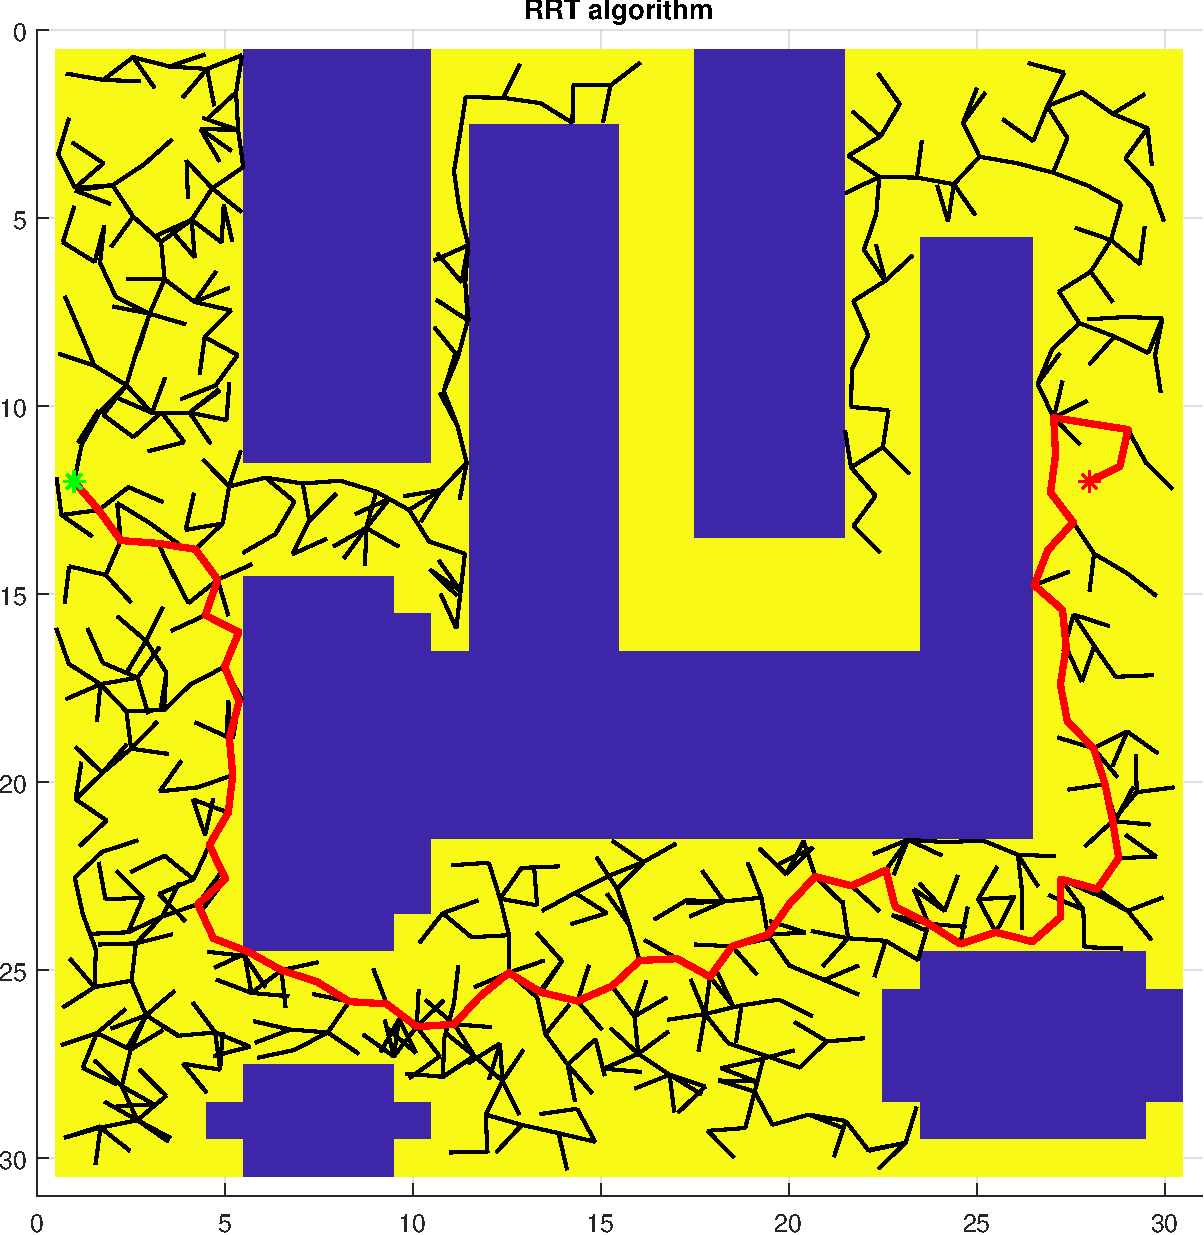
\includegraphics[width=0.48\textwidth]{./img/MATLAB/testing/01_RRT.pdf}
    \hspace{6pt}
    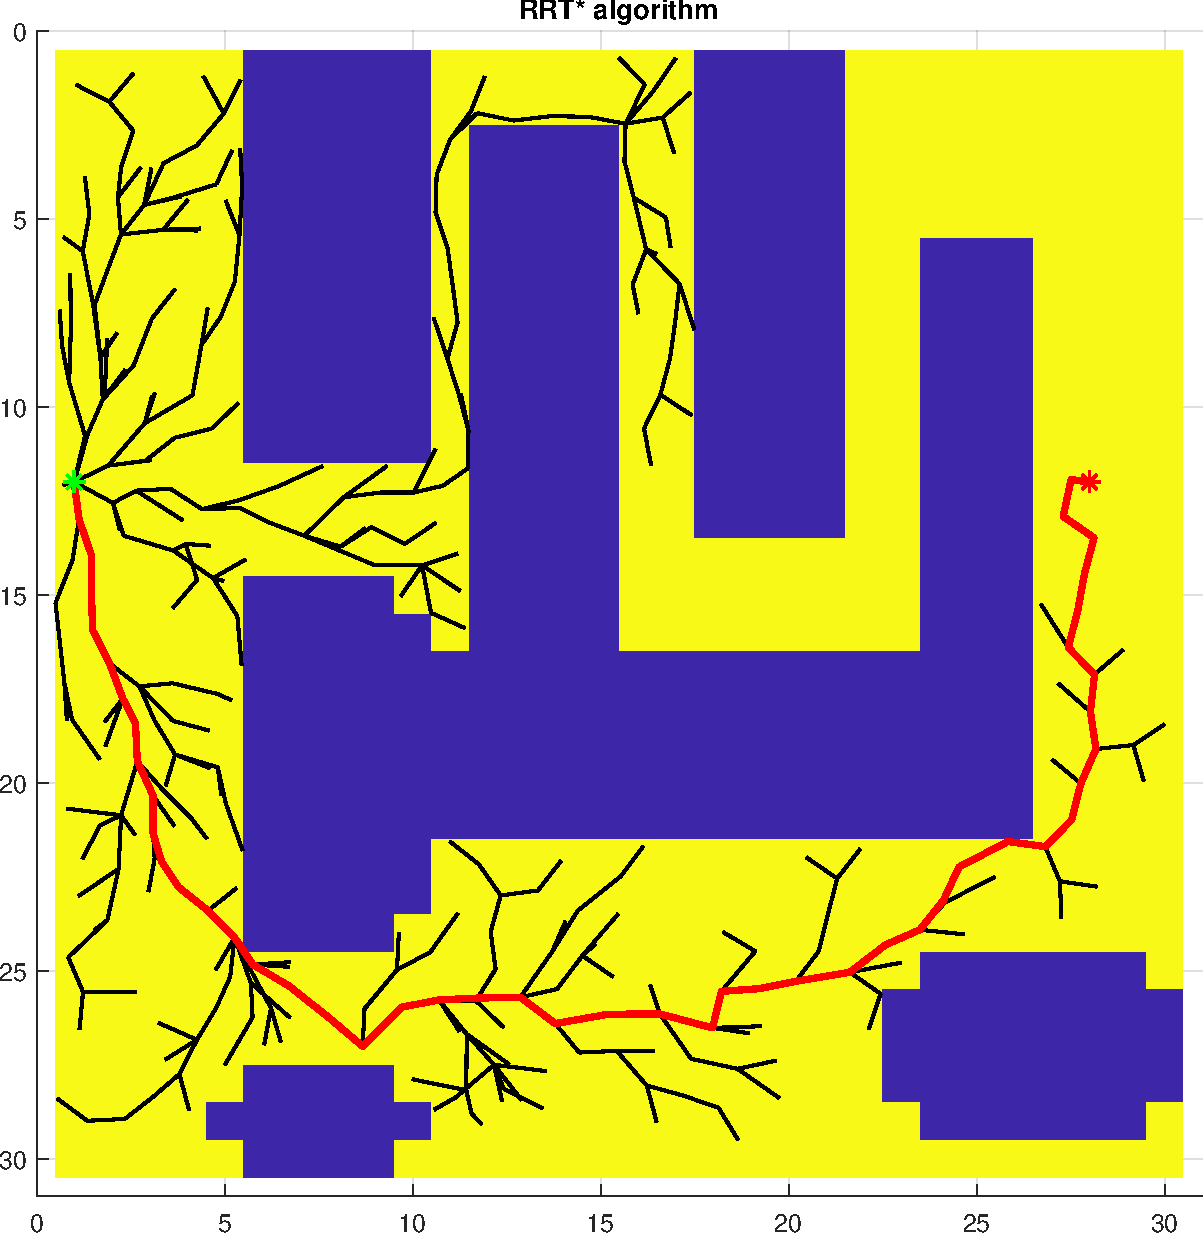
\includegraphics[width=0.48\textwidth]{./img/MATLAB/testing/01_RRT Star.pdf}

    \vspace{11pt}

    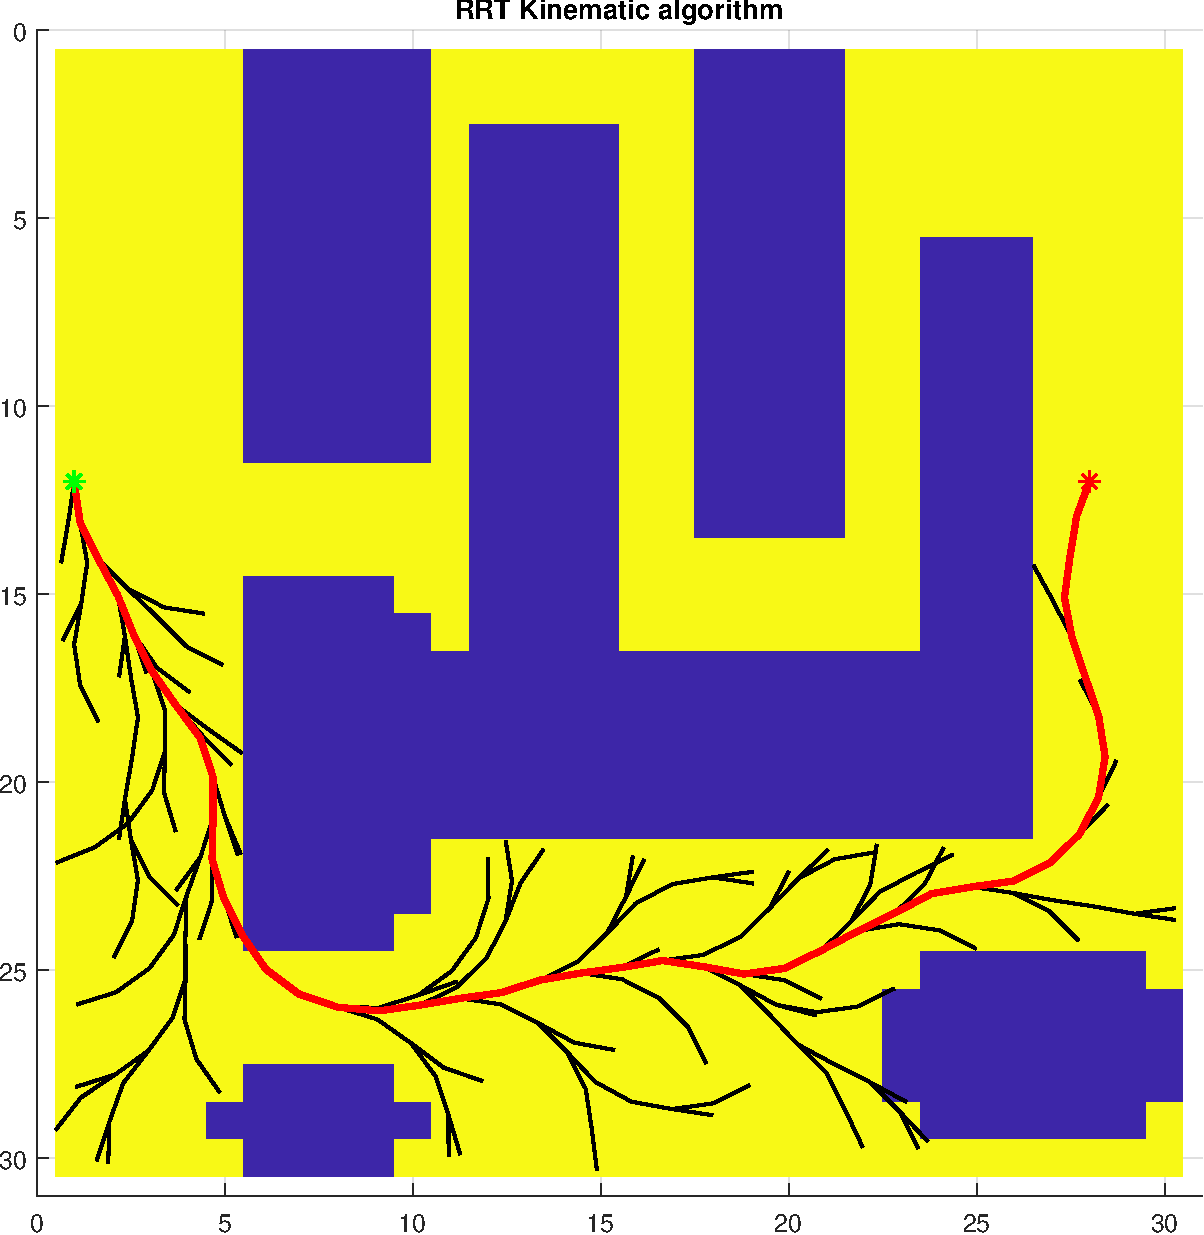
\includegraphics[width=0.48\textwidth]{./img/MATLAB/testing/01_RRT Kinematic.pdf}
    \hspace{6pt}
    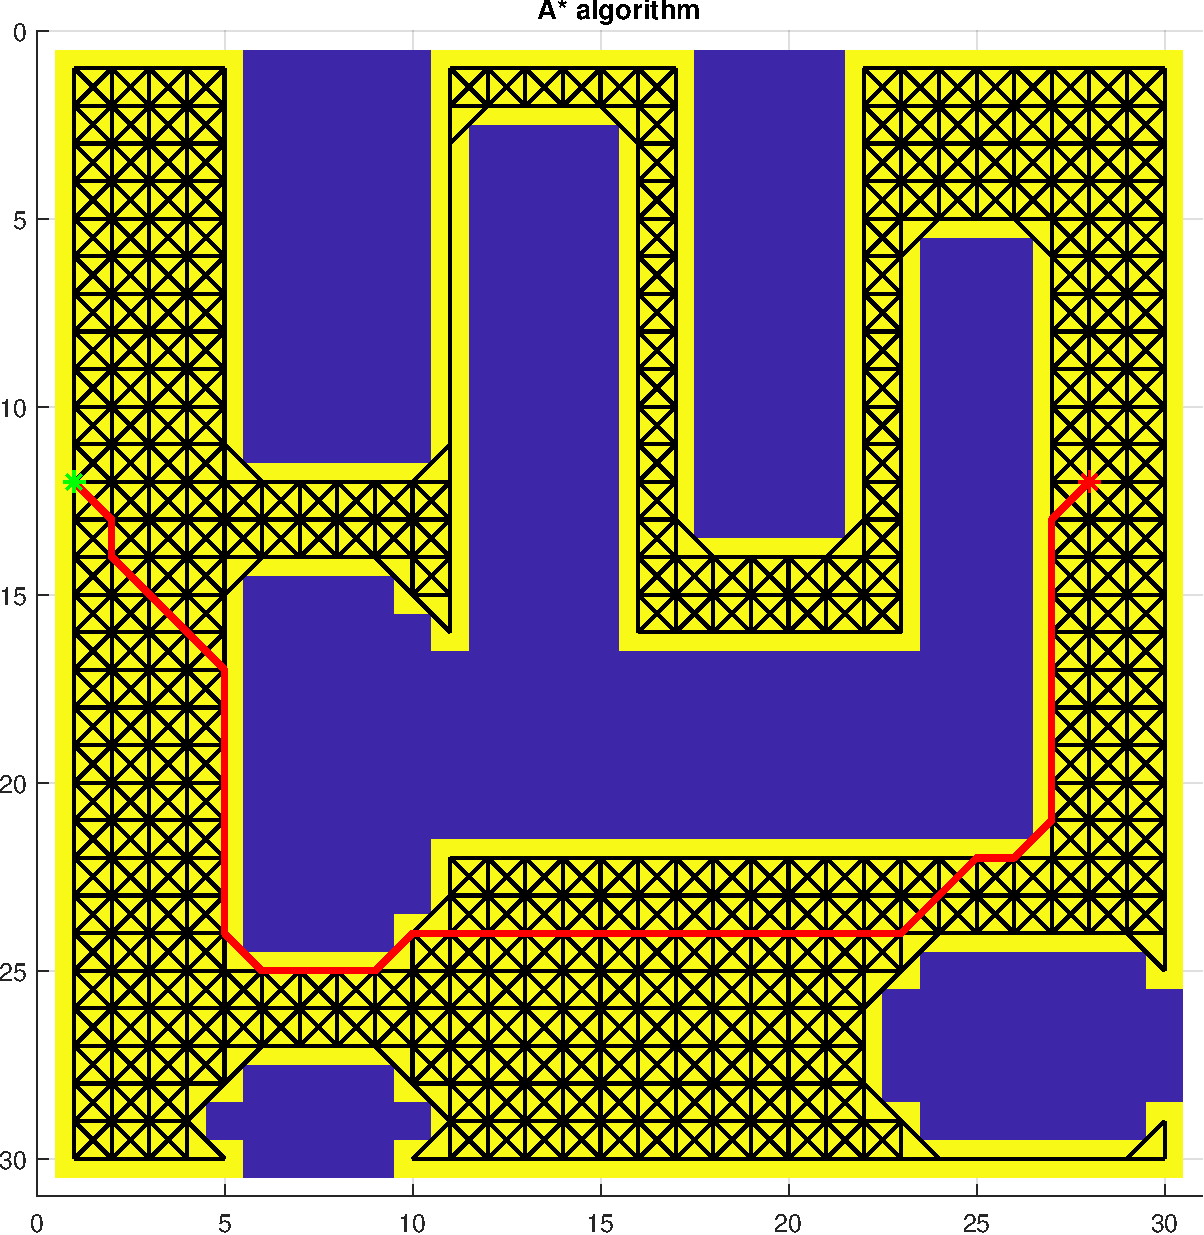
\includegraphics[width=0.48\textwidth]{./img/MATLAB/testing/01_A.pdf}
    \caption{Tree generated and path found by the RRT, RRT* and RRT Kinematic algorithms on map 1.}
    \label{fig:map_1_results}
\end{figure}

\begin{table}[H]
    \centering
    \begin{tabular}{|c|c|c|c|c|}
        \hline
        \textbf{Algorithm} & \textbf{Elapsed time (ms)} & \textbf{Tree dimension} & \textbf{Path length (m)} \\
        \hline
        RRT                & 145                        & 338                     & 57                       \\
        RRT*               & 202                        & 271                     & 49                       \\
        RRT Kinematic      & 129                        & 457                     & 49                       \\
        \hline
        A*                 & 1987                       & 3332                    & 47                       \\
        \hline
    \end{tabular}
    \caption{Results of the algorithms on map 1.}
    \label{tab:map_1_results}
\end{table}

The results clearly show the core problematics of the sampling-based algorithms: the path found is not optimal.

Comparing the results of the RRT and RRT* algorithms, we can see that the latter is able to find a shorter path, but it's still not able to reach the lower limit which is the one found by the A* algorithm.
On the other hand, sampling-based algorithms demonstrate to be in general $10$x faster than grid-based algorithms, as we can see from the elapsed time.
Also, under the space complexity point of view, the search space is significantly smaller for the sampling-based algorithms.
This suggests that the sampling-based algorithms are more efficient in terms of space complexity, as they do not need to explore the whole workspace to find a feasible path.


\subsubsection{Map 2}
\label{subsec:map_2}

Results obtained running the three algorithms on the second map are shown in Figures \ref{fig:map_2_results} and Table \ref{tab:map_2_results}.
The path found by the algorithm is shown in red, while the tree/graph is shown in black.
Again, we have included the results of the A* algorithm for comparison purposes.

\begin{figure}[H]
    \centering
    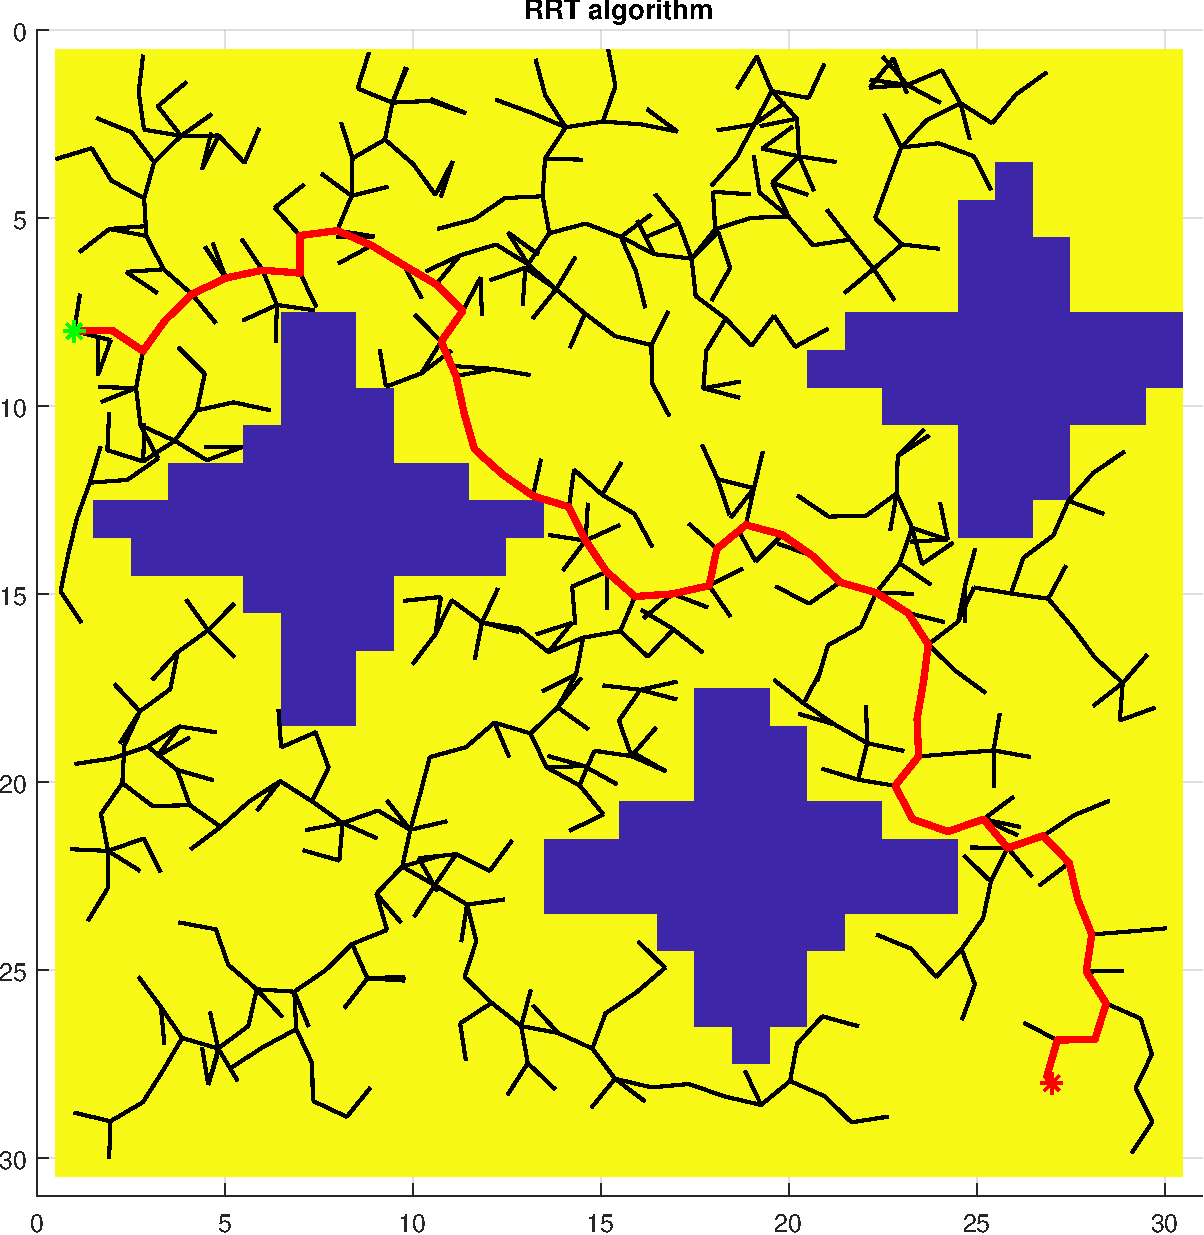
\includegraphics[width=0.48\textwidth]{./img/MATLAB/testing/02_RRT.pdf}
    \hspace{6pt}
    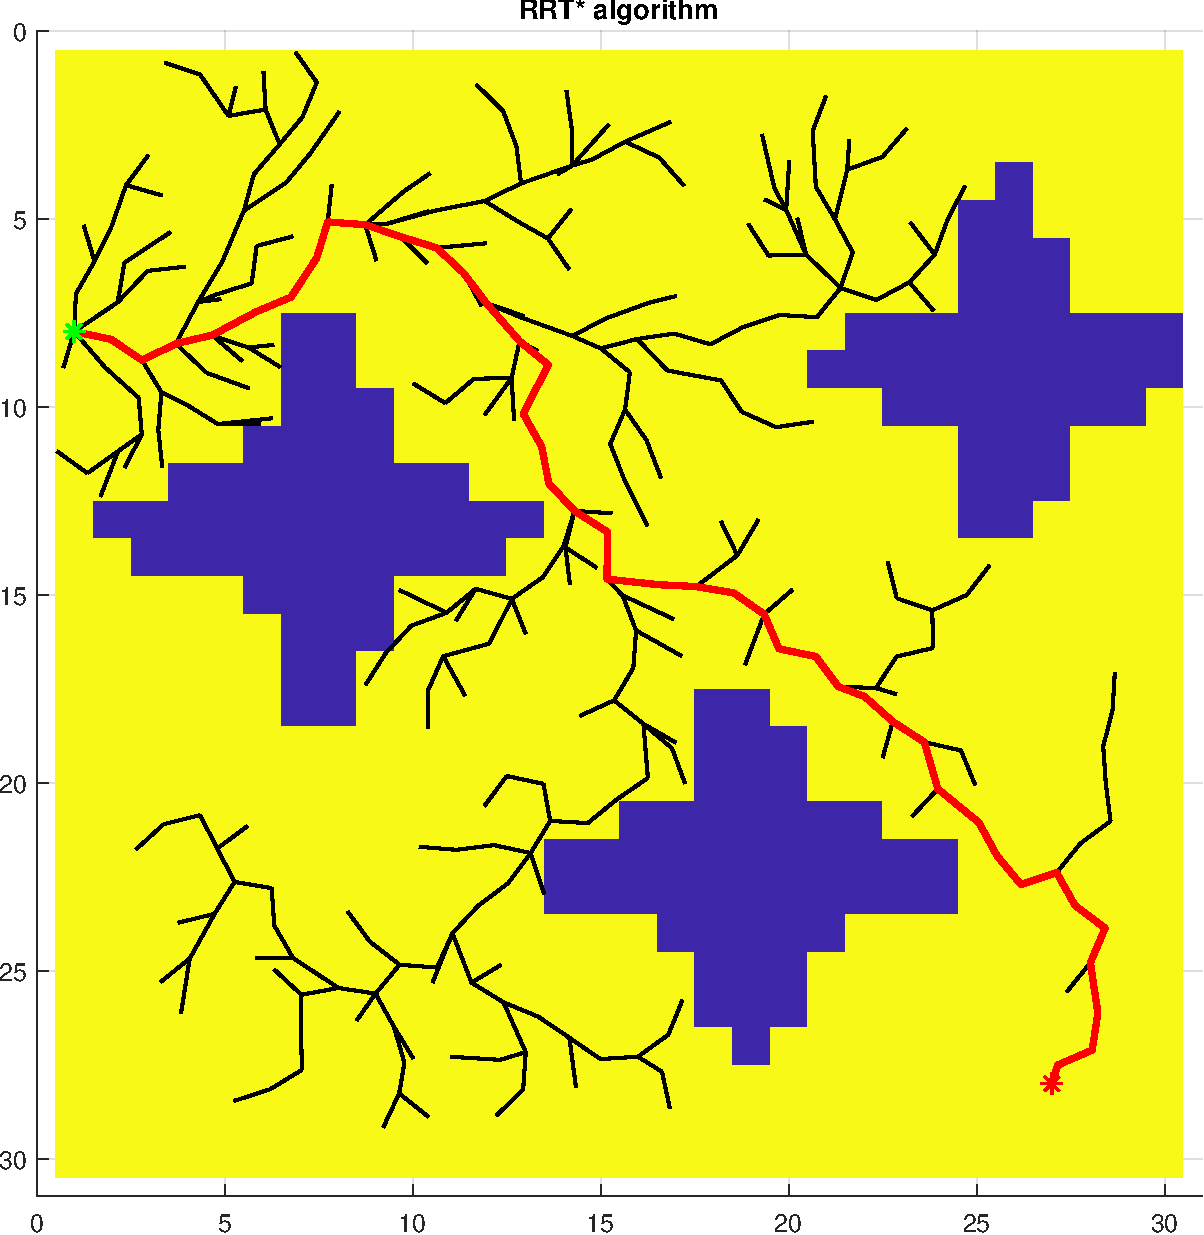
\includegraphics[width=0.48\textwidth]{./img/MATLAB/testing/02_RRT Star.pdf}

    \vspace{11pt}

    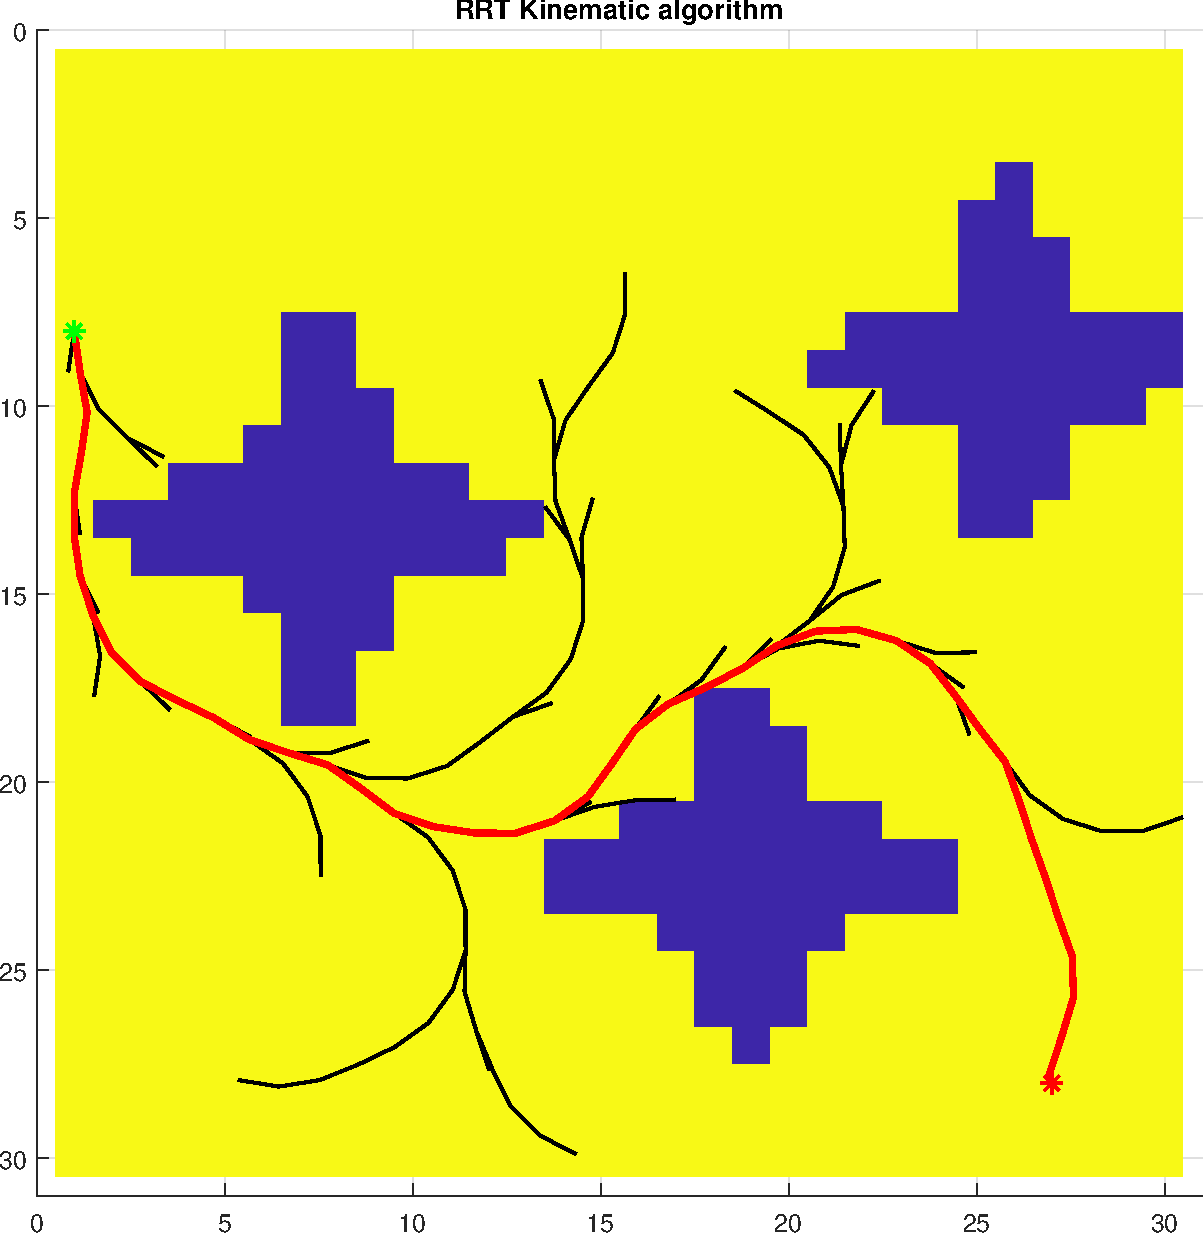
\includegraphics[width=0.48\textwidth]{./img/MATLAB/testing/02_RRT Kinematic.pdf}
    \hspace{6pt}
    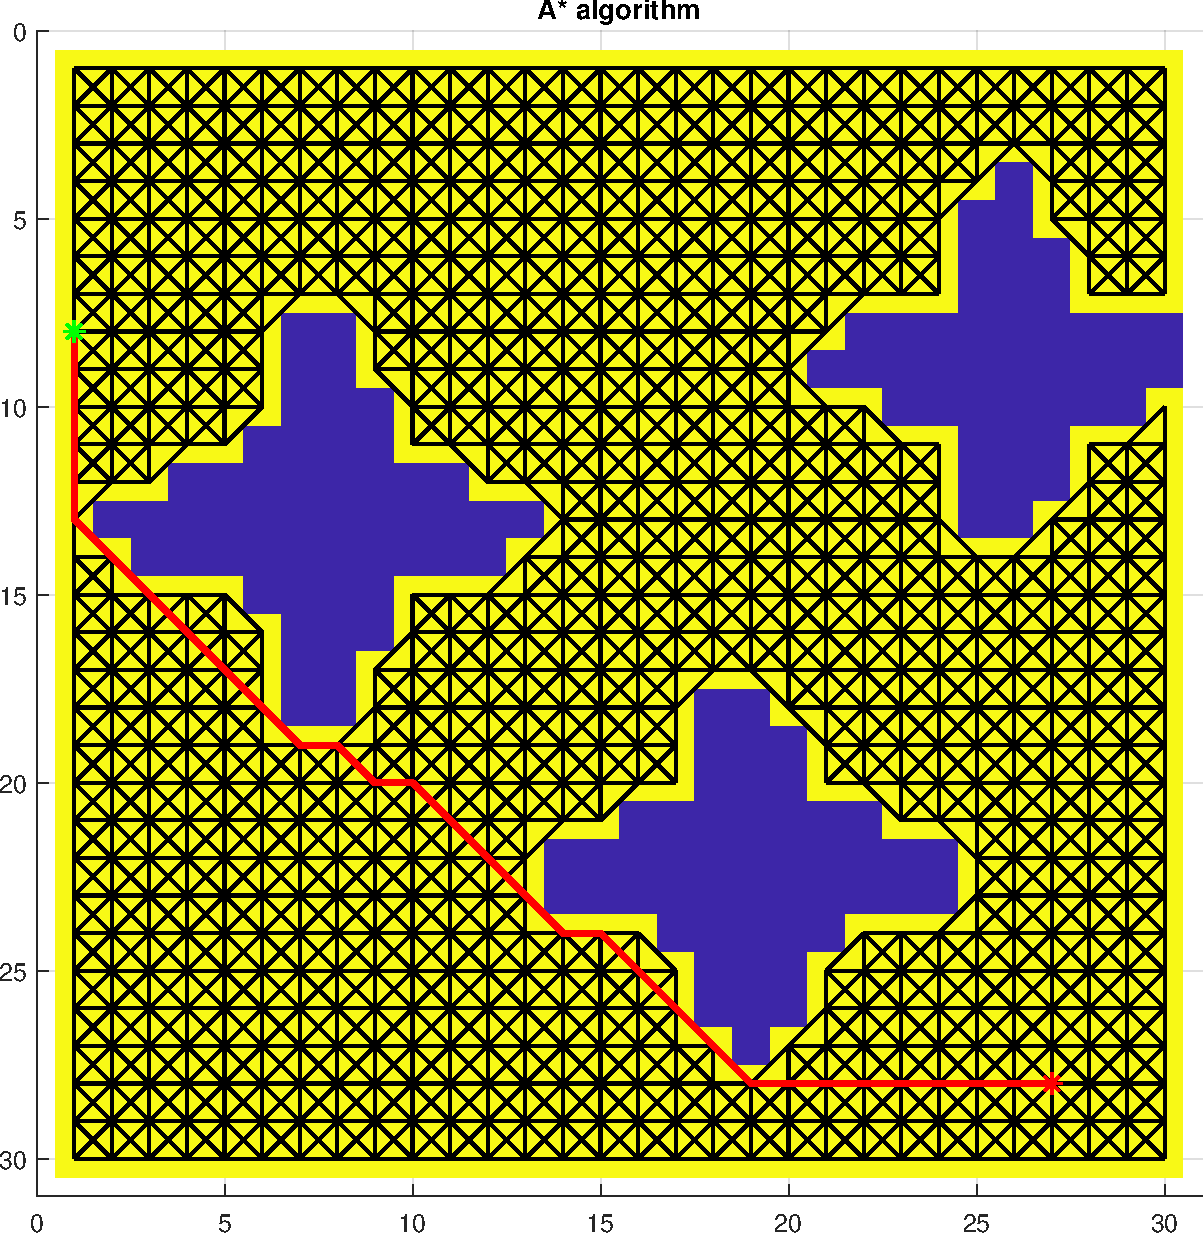
\includegraphics[width=0.48\textwidth]{./img/MATLAB/testing/02_A.pdf}
    \caption{Tree generated and path found by the RRT, RRT* and RRT Kinematic algorithms on map 2.}
    \label{fig:map_2_results}
\end{figure}

\begin{table}[H]
    \centering
    \begin{tabular}{|c|c|c|c|c|}
        \hline
        \textbf{Algorithm} & \textbf{Elapsed time (ms)} & \textbf{Tree dimension} & \textbf{Path length (m)} \\
        \hline
        RRT                & 199                        & 581                     & 49                       \\
        RRT*               & 360                        & 383                     & 40                       \\
        RRT Kinematic      & 282                        & 615                     & 42                       \\
        \hline
        A*                 & 2025                       & 5398                    & 37                       \\
        \hline
    \end{tabular}
    \caption{Results of the algorithms on map 2.}
    \label{tab:map_2_results}
\end{table}

Once again, we observe that the path found by the sampling-based algorithms is suboptimal.
Similar to before, the RRT* algorithm is the one able to get the closest to the optimal path found by the A* algorithm but still, it is not able to reach it.
As for the elapsed time, we still recognize a factor of around $8$ in speedup of the sampling-based algorithms with respect to the grid-based ones.
We also recall that this particular map and start/goal configuration is the one where the A* algorithm was able to find the optimal path in the shortest time, thanks to the heuristic adopted and the lower number of possible dead-ends-street during the search.
We believe that the speed-up factor might be even higher in more complex maps, where the A* algorithm would have to explore a larger number of nodes before finding the optimal path.


\subsubsection{Map 3}
\label{subsec:map_3}

Results obtained running the three algorithms on the third map are shown in Figures \ref{fig:map_3_results} and Table \ref{tab:map_3_results}.
The path found by the algorithm is shown in red, while the tree/graph is shown in black.
Again, we have included the results of the A* algorithm for comparison purposes.

\begin{figure}[H]
    \centering
    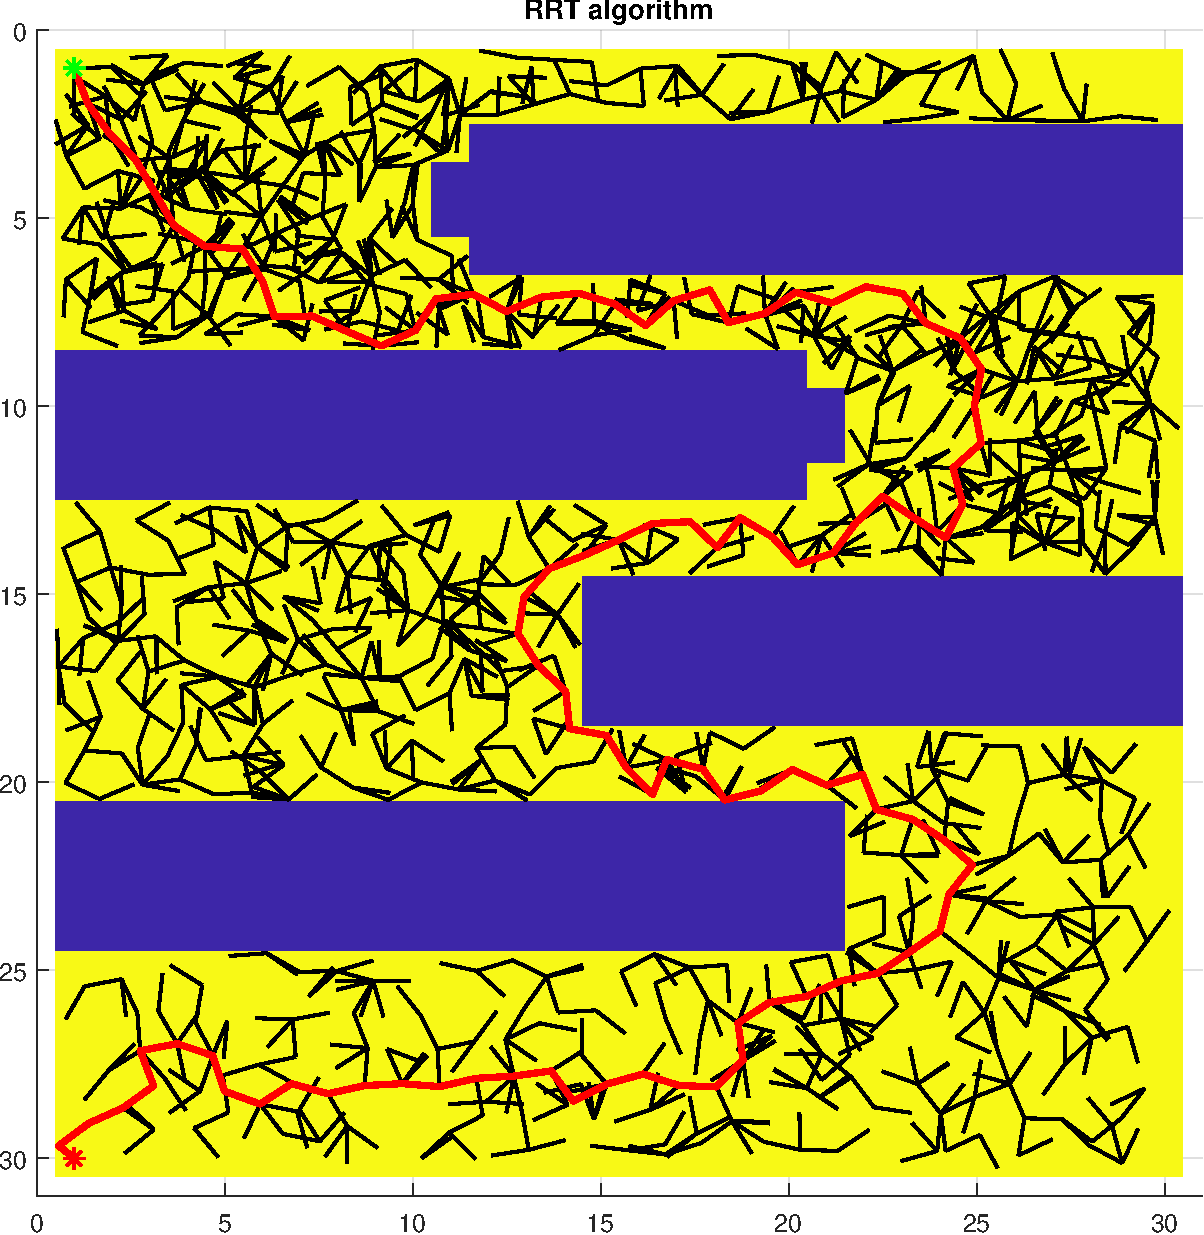
\includegraphics[width=0.48\textwidth]{./img/MATLAB/testing/03_RRT.pdf}
    \hspace{6pt}
    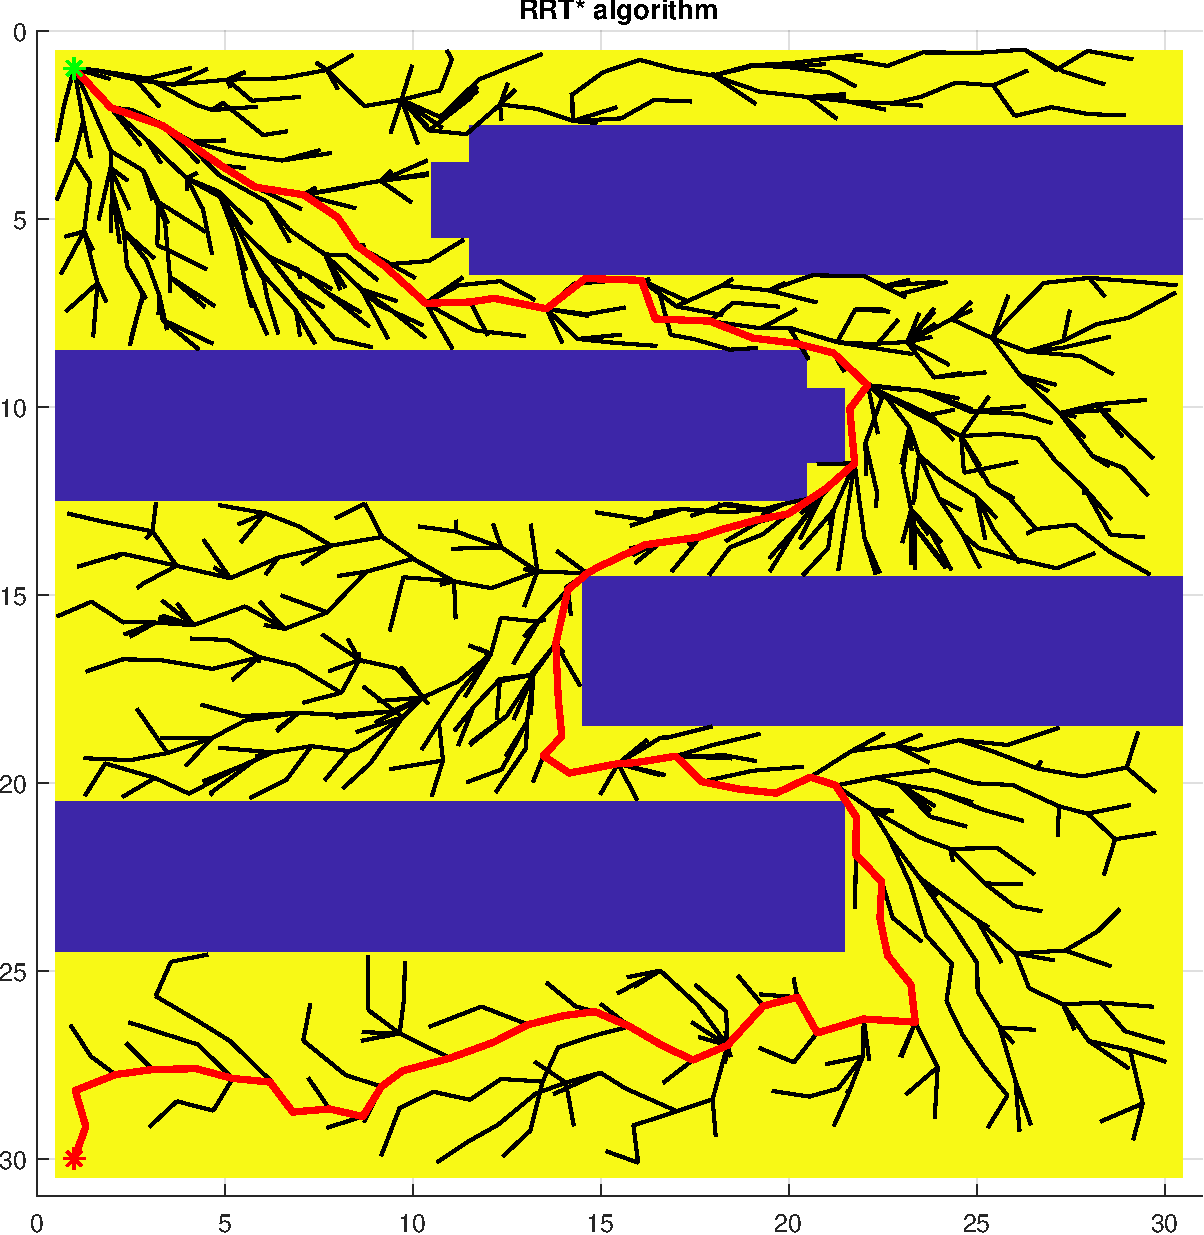
\includegraphics[width=0.48\textwidth]{./img/MATLAB/testing/03_RRT Star.pdf}

    \vspace{11pt}

    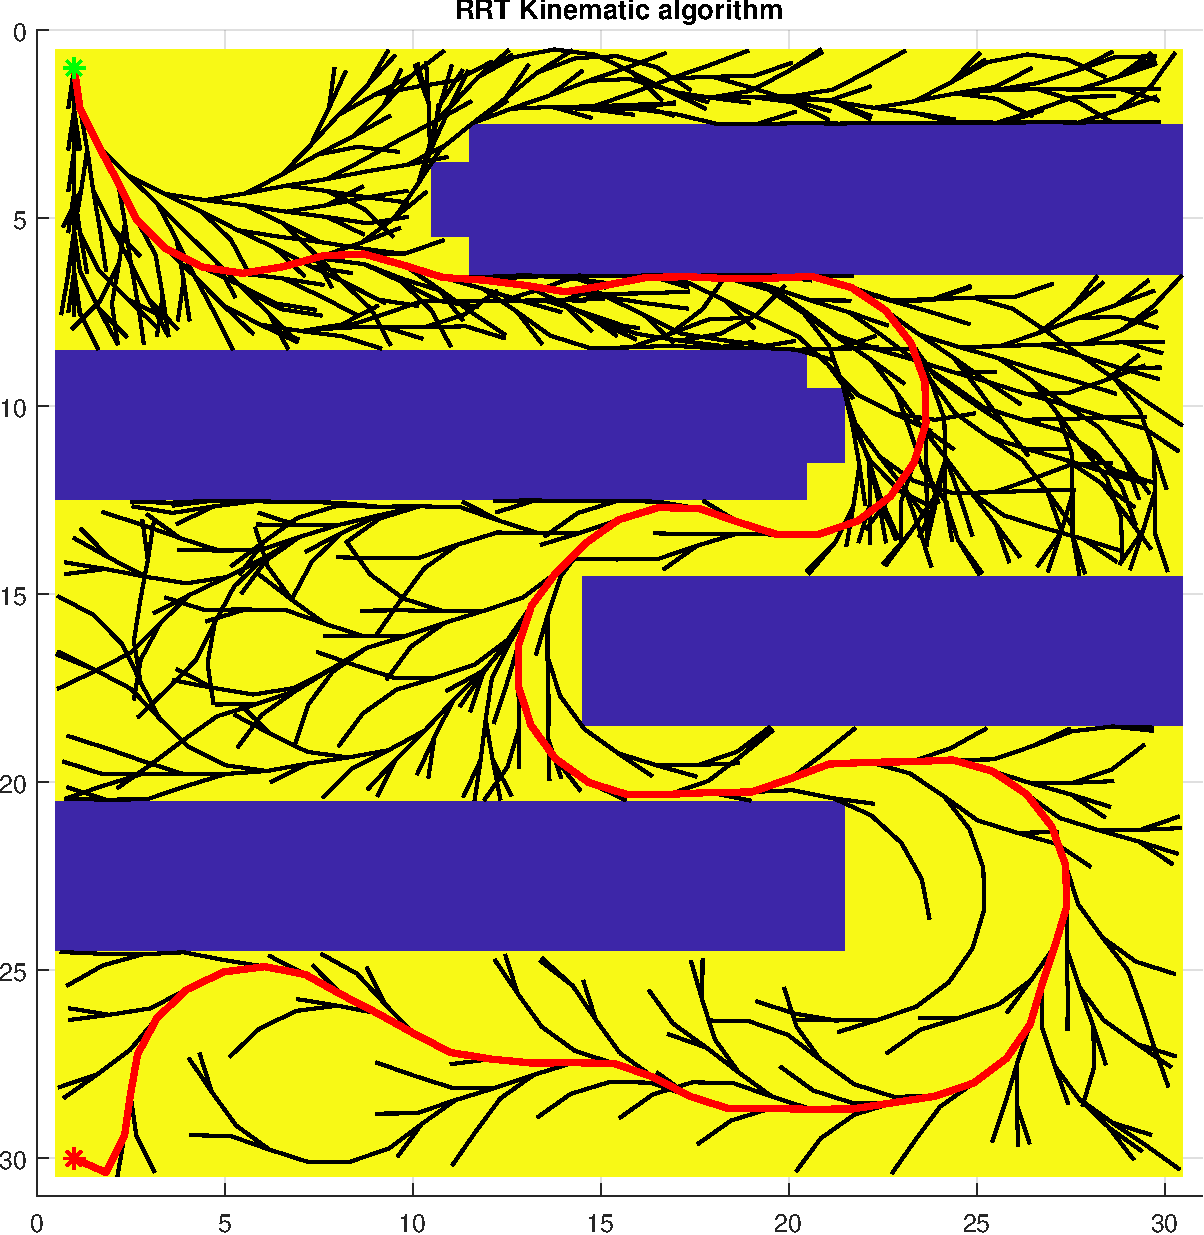
\includegraphics[width=0.48\textwidth]{./img/MATLAB/testing/03_RRT Kinematic.pdf}
    \hspace{6pt}
    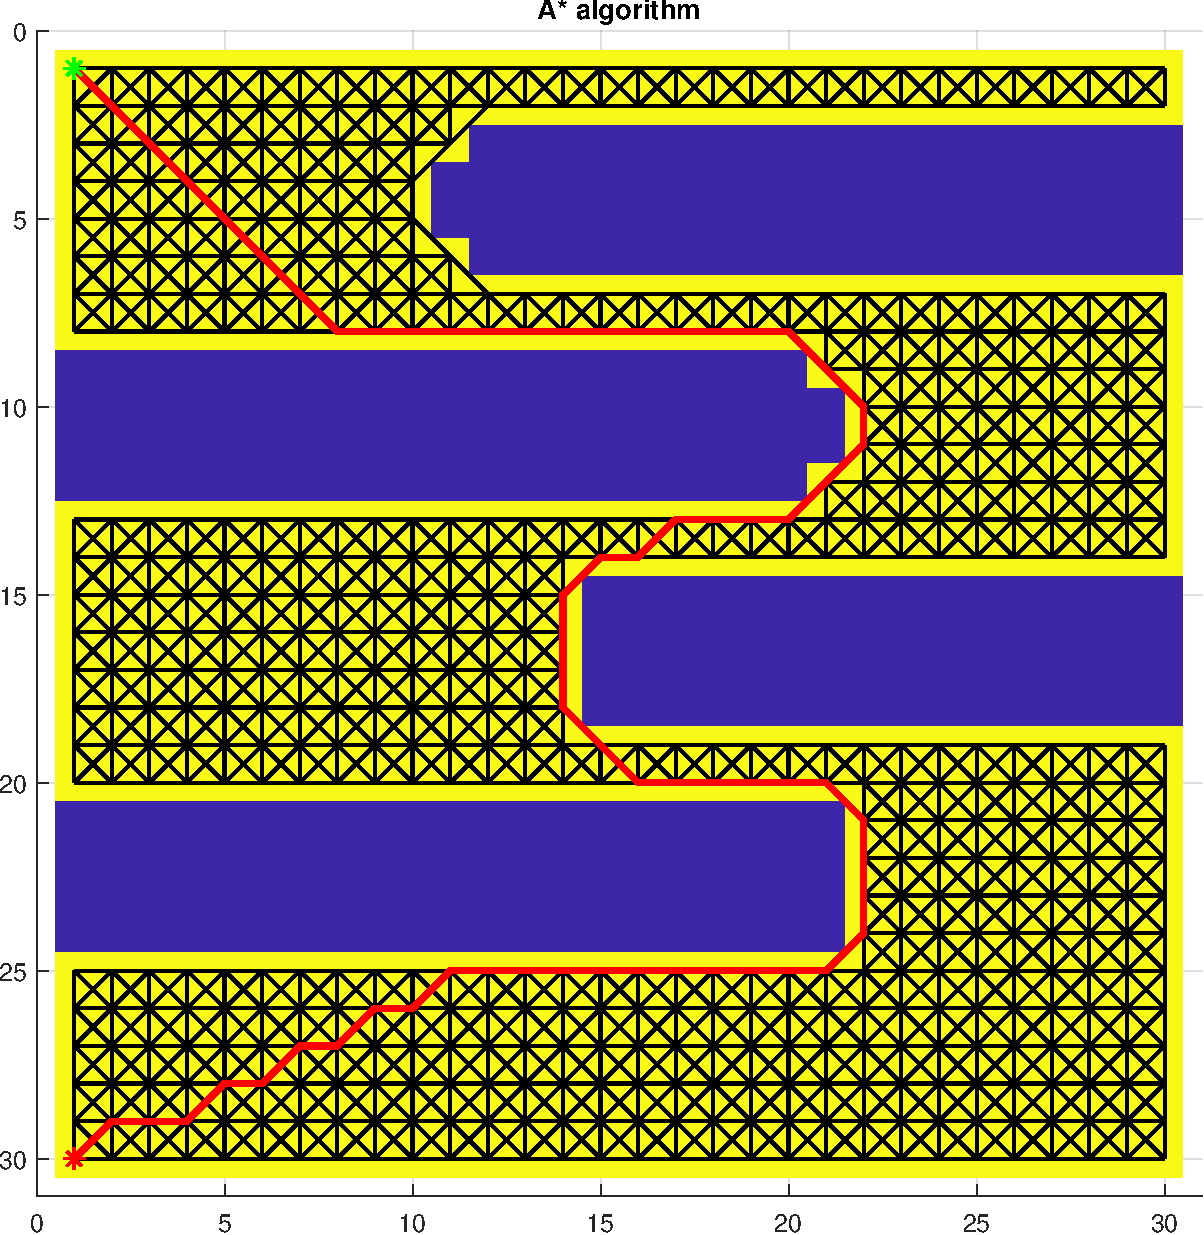
\includegraphics[width=0.48\textwidth]{./img/MATLAB/testing/03_A.pdf}
    \caption{Tree generated and path found by the RRT, RRT* and RRT Kinematic algorithms on map 3.}
    \label{fig:map_3_results}
\end{figure}

\begin{table}[H]
    \centering
    \begin{tabular}{|c|c|c|c|c|}
        \hline
        \textbf{Algorithm} & \textbf{Elapsed time (ms)} & \textbf{Tree dimension} & \textbf{Path length (m)} \\
        \hline
        RRT                & 552                        & 1085                    & 97                       \\
        RRT*               & 1208                       & 932                     & 74                       \\
        RRT Kinematic      & 68601                      & 10338                   & 93                       \\
        \hline
        A*                 & 2216                       & 3936                    & 74                       \\
        \hline
    \end{tabular}
    \caption{Results of the algorithms on map 3.}
    \label{tab:map_3_results}
\end{table}

From the test performed on this map, we gain further information about the performance of the algorithms in cluttered environments.
In this case, the difference in computation time between the sampling-based algorithms and the A* algorithm is not as significant as in the previous cases.
The sampling approach is in fact heavily slowed down by the four obstacles, that impose the need of numerous samples to progress in the successive sectors of the map up to the goal.
This is also reflected in the distribution of the nodes in the tree, which is much denser in the upper sectors of the map (near the starting point) than in the lower ones (near the goal).
RRT-kinematic clearly shows this behavior, highlighting the trapping of the algorithm in front of each obstacle.
A* algorithm, on the other hand, still suffers from local dead-ends searching, but it's much quicker in finding a way to get around the obstacles.

For completeness, we also report that in the case of the RRT-kinematic algorithm, high variance in the results was observed.
In particular, among the runs performed, we have one case where the algorithm was able to find a path in $8.6$ seconds, while in the worse case it took $115.7$ seconds.



\subsubsection{Map 4}
\label{subsec:map_4}

Results obtained running the three algorithms on the fourth map are shown in Figures \ref{fig:map_4_results} and Table \ref{tab:map_4_results}.
The path found by the algorithm is shown in red, while the tree/graph is shown in black.
Again, we have included the results of the A* algorithm for comparison purposes.

\begin{figure}[H]
    \centering
    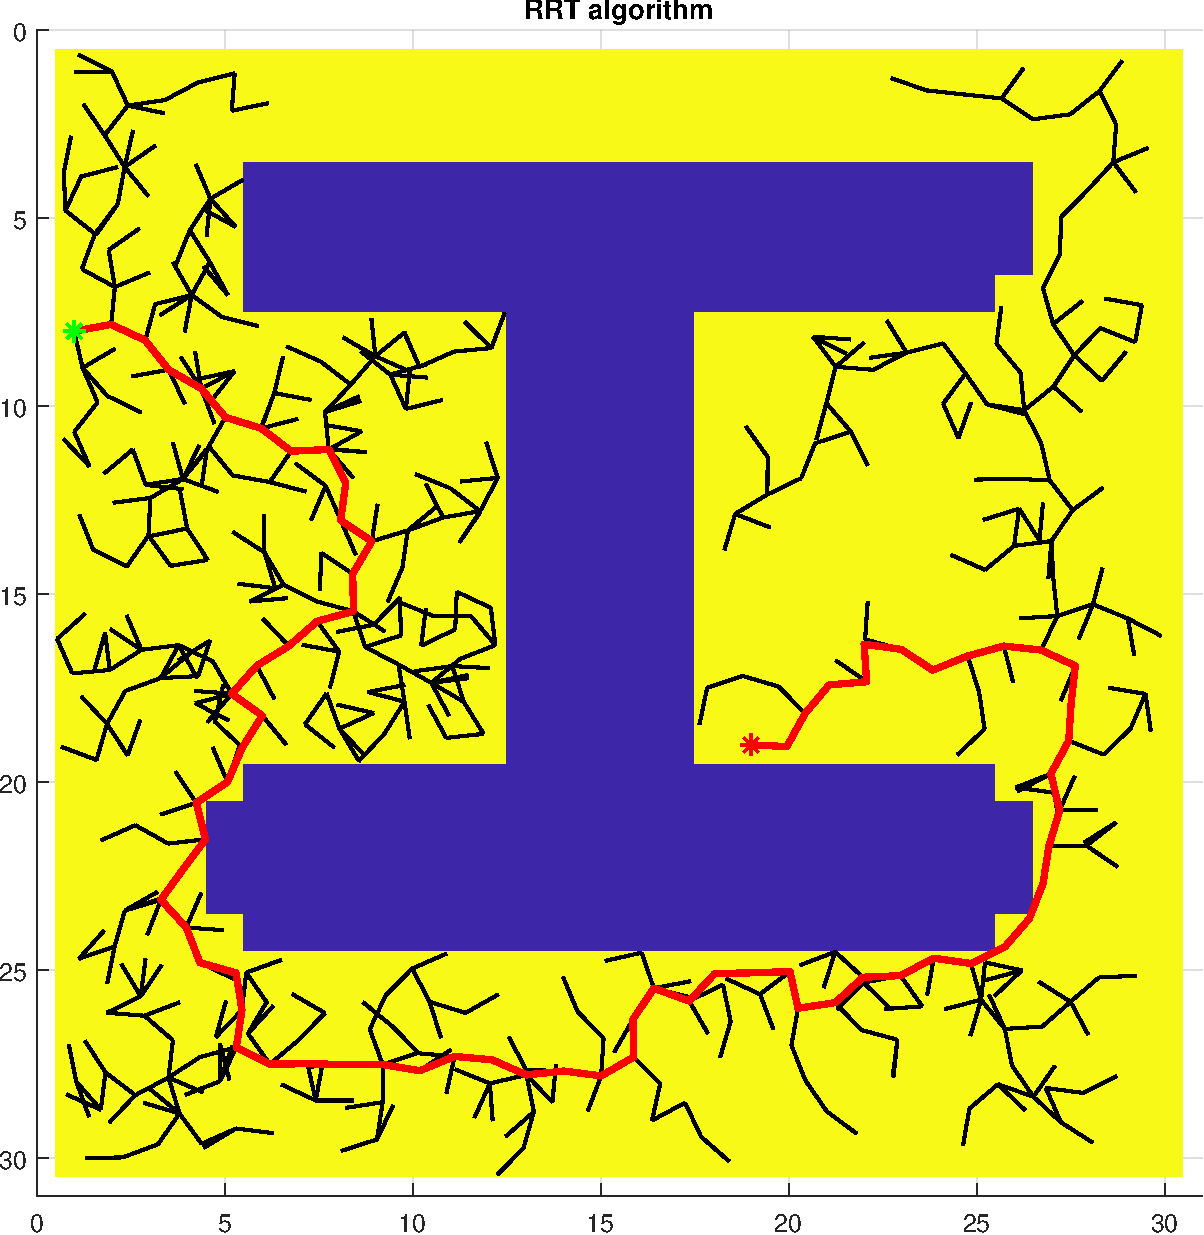
\includegraphics[width=0.48\textwidth]{./img/MATLAB/testing/04_RRT.pdf}
    \hspace{6pt}
    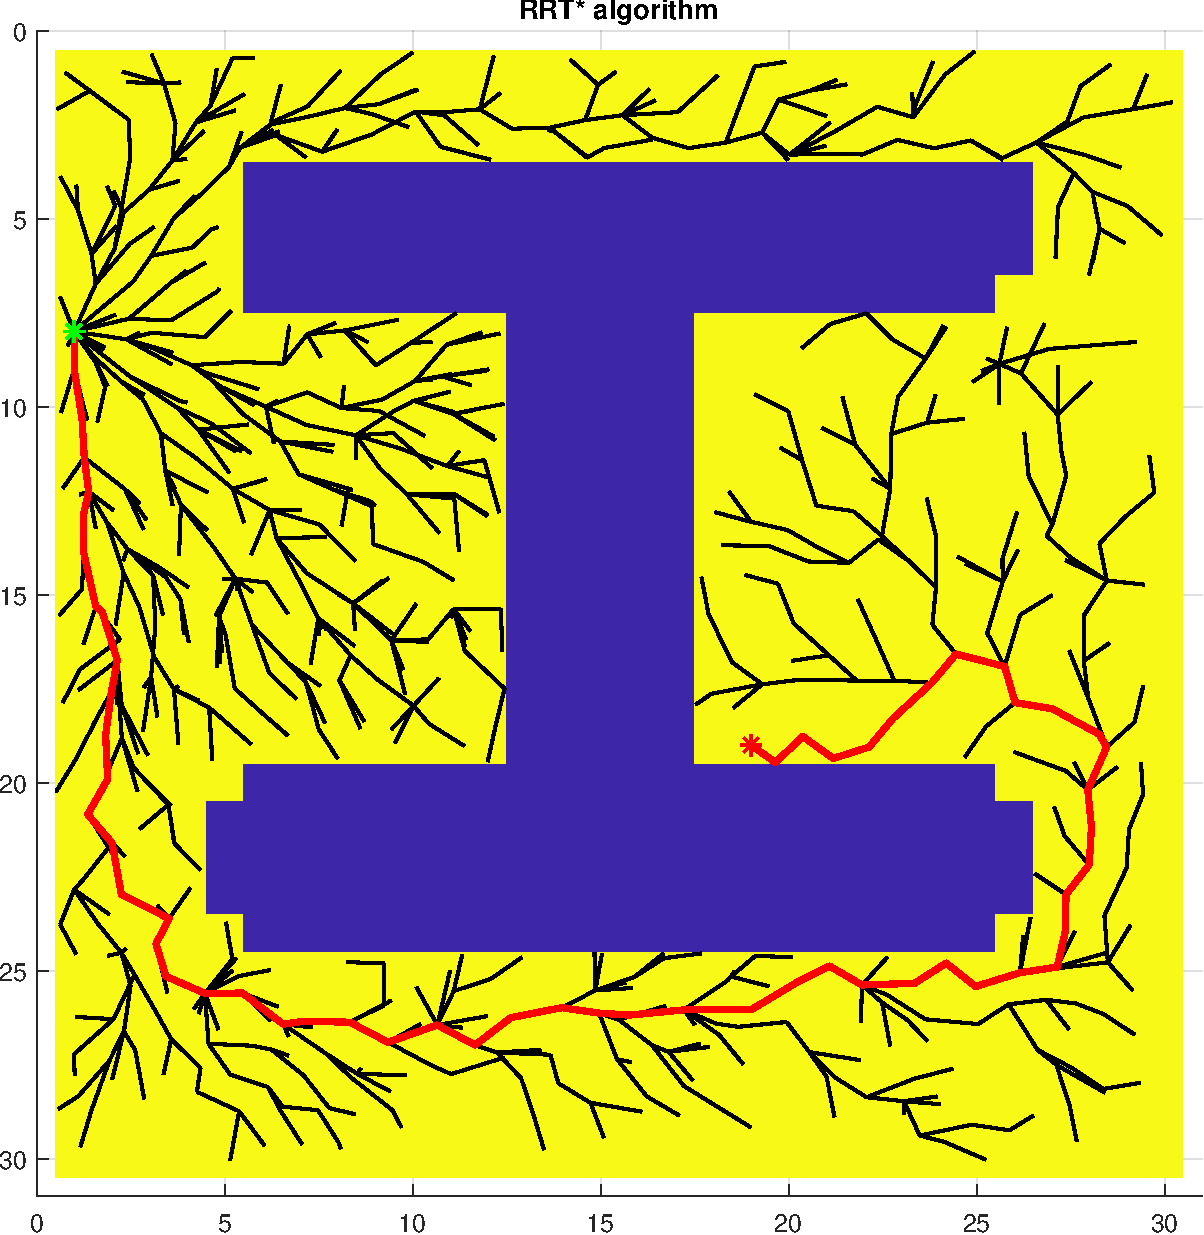
\includegraphics[width=0.48\textwidth]{./img/MATLAB/testing/04_RRT Star.pdf}

    \vspace{11pt}

    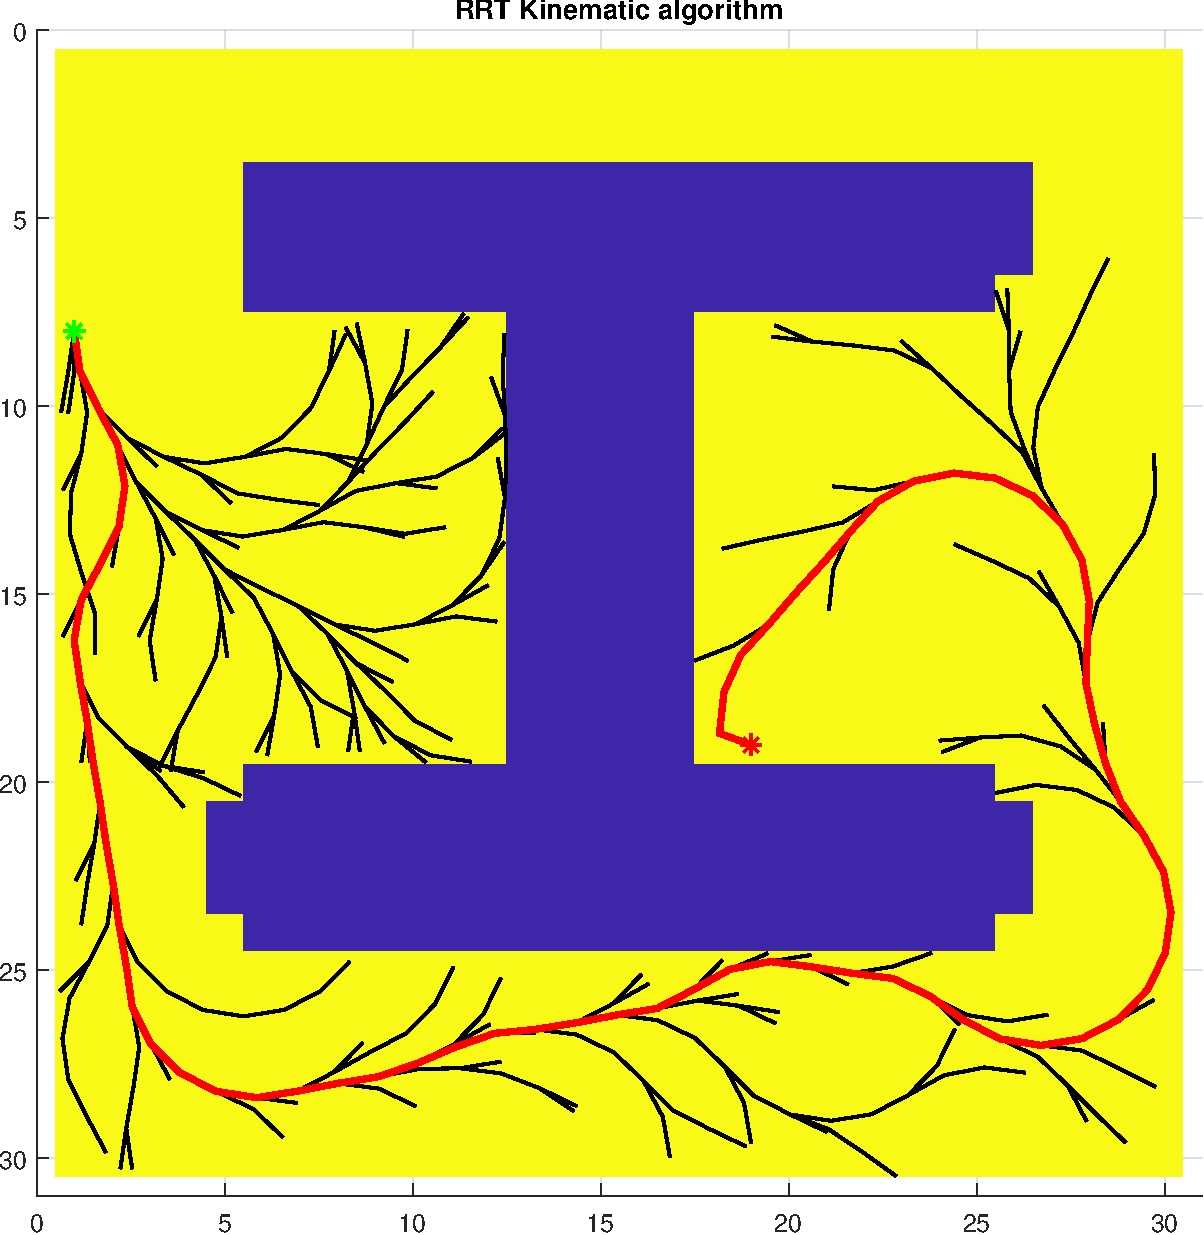
\includegraphics[width=0.48\textwidth]{./img/MATLAB/testing/04_RRT Kinematic.pdf}
    \hspace{6pt}
    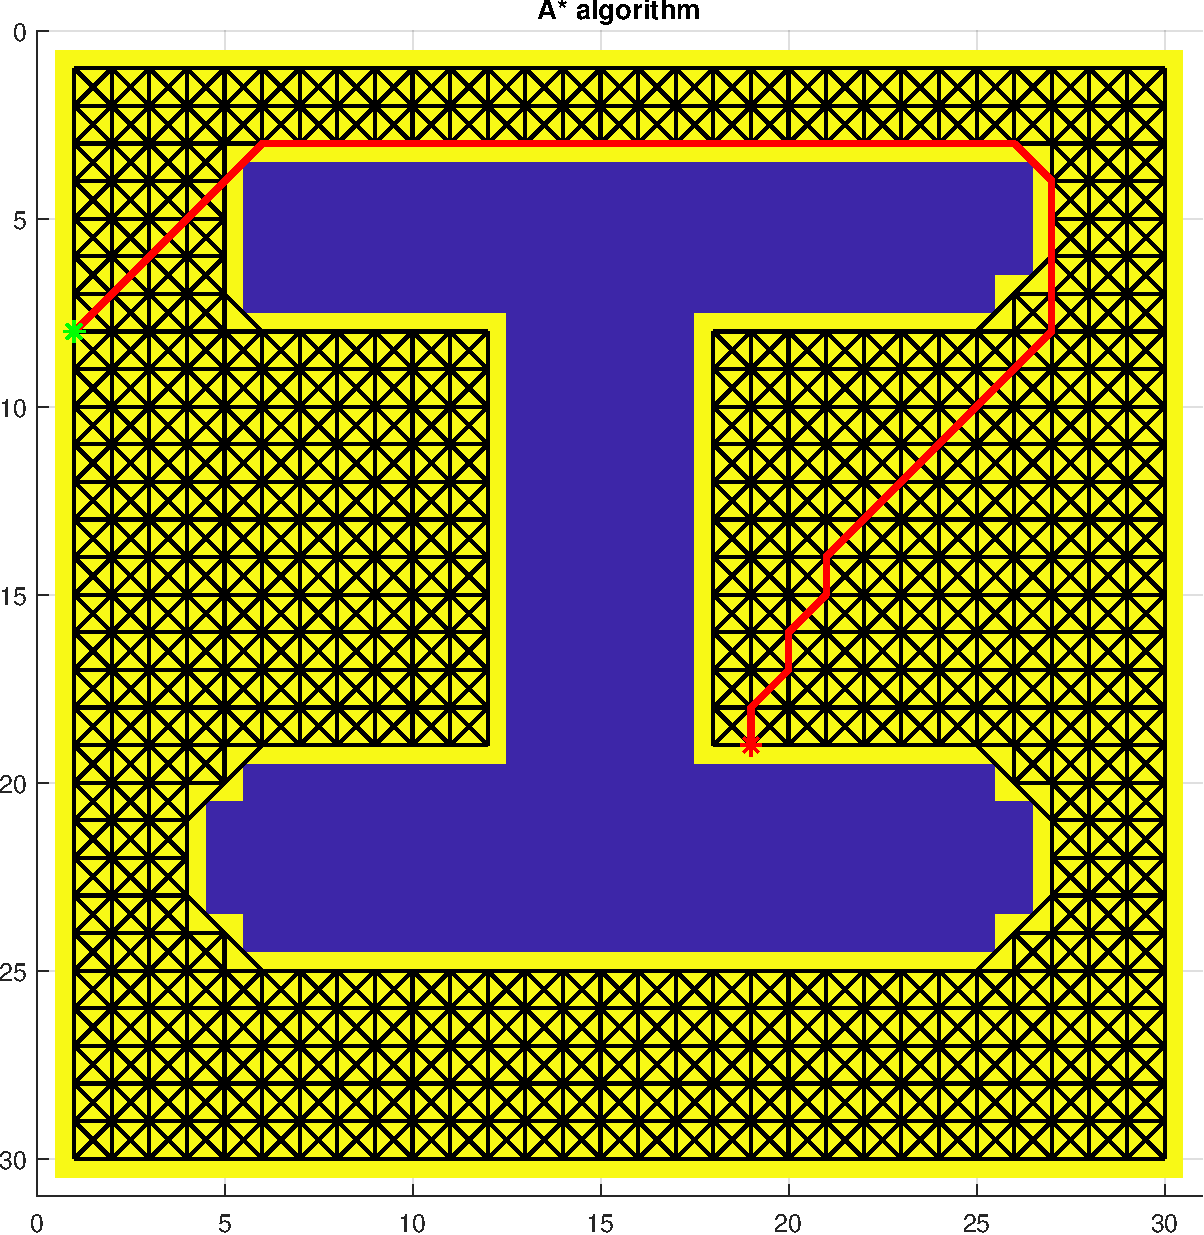
\includegraphics[width=0.48\textwidth]{./img/MATLAB/testing/04_A.pdf}
    \caption{Tree generated and path found by the RRT, RRT* and RRT Kinematic algorithms on map 4.}
    \label{fig:map_4_results}
\end{figure}

\begin{table}[H]
    \centering
    \begin{tabular}{|c|c|c|c|c|}
        \hline
        \textbf{Algorithm} & \textbf{Elapsed time (ms)} & \textbf{Tree dimension} & \textbf{Path length (m)} \\
        \hline
        RRT                & 164                        & 604                     & 67                       \\
        RRT*               & 485                        & 618                     & 45                       \\
        RRT Kinematic      & 782                        & 1649                    & 64                       \\
        \hline
        A*                 & 2607                       & 4520                    & 47                       \\
        \hline
    \end{tabular}
    \caption{Results of the algorithms on map 4.}
    \label{tab:map_4_results}
\end{table}

The results obtained on this map are similar to the ones obtained on the previous ones.
It's interesting to notice how the RRT was not able to explore the upper region of the map, in which instead the A* finds its optimal path.
Once again, the concept of obstacles blocking the path of the sampling-based algorithms is highlighted similarly to the previous case.